\documentclass[english]{ltugboat}
\usepackage{babel}
\usepackage[T1]{fontenc}
\usepackage{multicol}
\usepackage{calc}
\usepackage[simplified]{pgf-umlcd}
\usetikzlibrary{calc}
\usepackage{graphicx}
\usepackage{microtype}
\usepackage[hidelinks,pdfa]{hyperref}
\usepackage{listings}
% For colored variants see:
%   https://github.com/Xerdi/texmf-packaging
%\usepackage{lstlangjson}
%\usepackage{lstlangyaml}
\usepackage{subcaption}
\usepackage{ulem}
\usepackage{wasysym}
\usepackage{dirtree}
\title{Specifying and Populating Documents in YAML with lua-placeholders in LaTeX}

% repeat info for each author; comment out items that don't apply.
\author{Erik Nijenhuis}
\address{Frans Halsstraat 38\\ Leeuwarden, 8932 JC \\ The Netherlands}
\netaddress{erik (at) xerdi dot com}
\personalURL{https://github.com/MacLotsen}
%\ORCID{0}
% To receive a physical copy of the TUGboat issue, please include the
% mailing address we should use, as a comment if you prefer it not be printed.

% Tikz setup
\renewcommand{\umltextcolor}{black}
\renewcommand{\umlfillcolor}{white}
\renewcommand{\umldrawcolor}{black}

\def\pkg#1{\texttt{#1}}

\lstset{
    columns=fullflexible,
    basicstyle=\ttfamily,
    keywordstyle={\bfseries},
    keywordstyle=[2]{\bfseries},
    commentstyle={\itshape},
    stepnumber=1,
    numbersep=5pt,
    numberstyle=\ttfamily,
    showspaces=false,
    showstringspaces=false,
    showtabs=false,
    tabsize=4,
    breaklines=true,
    breakatwhitespace=false
}

% Style shorthands
\lstdefinestyle{tex}{
    language={[LaTeX]TeX}
}

\lstdefinestyle{yaml}{
    language=yaml
}

\lstdefinestyle{json}{
    language=json
}

\begin{document}
    \maketitle

    \begin{abstract}
    This article demonstrates how document variables are specified and supplied using YAML and describes how this can then assist in system integration using an open-source invoice application.
\end{abstract}

    \section*{Keywords}
    \LuaLaTeX, YAML

    \section{Inleiding}
Tijdens mijn werk als Software Engineer werd ik geconfronteerd met een uitdaging voor een bedrijf wat overeenkomsten en voorwaarden opstelt voor meerdere klanten.
Een lastige uitdaging daarin was het gescheiden houden van de klantgegevens en regelgevende documentatie.
Dit kan, zoals ik eerder had toegepast in GinVoice\cite{ginvoice}, door extra \LaTeX-bestanden te genereren met Python waardoor vervolgens het \LaTeX-hoofdbestand gecompileerd kan worden.
Echter, dit maal was mijn doel om een oplossing te bieden vanuit het \LaTeX-domein zelf, in plaats van het applicatiedomein.
De oplossing die ik daarvoor heb geschreven heet tegenwoordig \pkg{lua-placeholders}\cite{lua-placeholders} en introduceert een gedeelde datalaag met YAML tussen \LaTeX\ en applicatie code.
Het pakket biedt een tussenlaag, speciaal bedoeld voor data, door middel van YAML-bestanden.
Om deze oplossing te demonstreren pakken we GinVoice.
Dit voorbeeld, een Python GTK-applicatie die facturen genereert met \LaTeX, biedt net wat meer complexiteit en uitdagingen dan het juridisch domein te bieden heeft.

\subsection{De Compiler -- \LuaLaTeX}
Mijn beslissing om \LuaLaTeX\ als compiler te gebruiken, had meerdere redenen.
Sinds 2016 maak ik gebruik van \LuaLaTeX, wat me destijds voor documenten binnen de computerwetenschap enorm heeft geholpen.
In alle afgelopen jaren heb ik veel ervaring opgedaan in het compileren met \LuaLaTeX\ en zie ik het als ontwikkelaar als een geschikte compiler, dankzij de mogelijkheid om in Lua te scripten, wat ik als programmeur uiteraard enorm waardeer.

De mogelijkheid om in Lua te scripten biedt een aantal voordelen.
Het stelt mij in staat om complexe taken uit te voeren tijdens het compileerproces, zoals het verwerken van YAML-bestanden of het manipuleren en structureren van gegevens.
Bovendien biedt \LuaLaTeX\ ondersteuning voor Lua init scripts, waarmee ik een aangepast compilatieproces kan implementeren met een eigen CLI (Command Line Interface), waardoor het integratieproces nog verder wordt vereenvoudigd en geoptimaliseerd voor eindoplossingen.

\subsection{Wat is YAML?}
Als DevOps Engineer ben ik vaak YAML tegengekomen bij het werken met tools zoals Docker Compose, Travis CI, GitHub Actions en NetPlan van Canonical (Ubuntu systemen).
YAML wordt veel gebruikt in de DevOps-wereld voor het automatiseren en beheren van configuraties, waarbij het functioneert als een gestructureerde opmaaktaal voor het definiëren van configuratiebestanden en het vastleggen van infrastructurele en operationele aspecten van softwaretoepassingen.

YAML is een cruciaal onderdeel geworden van moderne softwareontwikkeling en -implementatie, vanwege zijn eenvoudige syntaxis en flexibiliteit.
In combinatie met \LaTeX\ biedt YAML een krachtig mechanisme om gestructureerde gegevens te definiëren en te beheren, wat vooral handig is bij het integreren van klantgegevens in \LaTeX-documenten.
In listing~\ref{lst:example} is een voorbeeld van YAML te zien in combinatie met \LaTeX.

\begin{lstlisting}[language=YAML,caption={\ttfamily invoice-001.yaml},label={lst:example}]
supplier: grapefruit
client: juicing-joker
title: Grapefruit Inc. Invoice
subtitle: for fruits and stuff
currency: \$
number: 1
date: \today
...
\end{lstlisting}
%Dit YAML-voorbeeld wordt verder besproken in hoofdstuk~\ref{sec:output}.

%Dit YAML-voorbeeld toont een specificatie van het veld \meta{message}, dat een standaardwaarde heeft voor een factuurtekst.
%De factuurtekst bevat variabelen zoals het bedrag, het factuurnummer en de naam van de leverancier, die worden ingevuld met behulp van het \pkg{lua-placeholders} pakket tijdens het compilatieproces van het \LaTeX-document.

%\subsection{De Scope van dit Artikel}\label{sec:scope}
%Om een goed voorbeeld te geven van de features en toegevoegde waarde van \pkg{lua-placeholders} nemen we de \LaTeX-factuur van GinVoice als uitgangspunt.
%
%\noindent
%\begin{figure}[!ht]
%    \centering
%    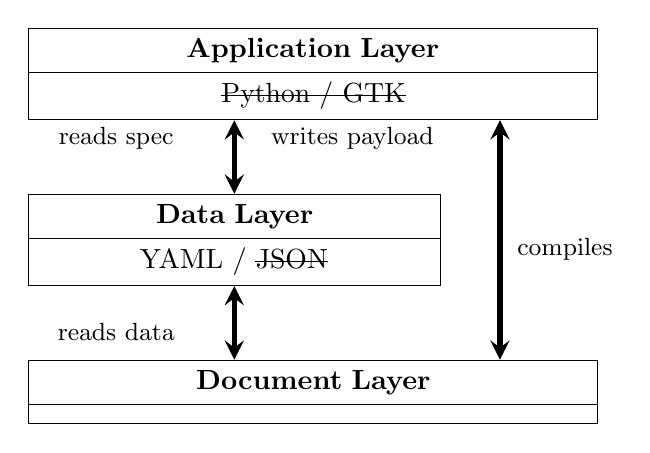
\begin{tikzpicture}[align=center]
    \begin{class}[text width=7cm]{Application Layer}{0,0}
        \attribute{\sout{Python / GTK}}
    \end{class}
    \begin{class}[text width=5cm]{Data Layer}{-1cm,-6em}
        \attribute{YAML / \sout{JSON}}
    \end{class}
    \begin{class}[text width=7cm]{Document Layer}{0,-12em}
        \attribute{\LuaLaTeX}
    \end{class}
    \draw[line width=2pt,{stealth}-{stealth}] ($(Application Layer.south) + (-1cm,0)$) to (Data Layer.north);
    \draw[line width=2pt,{stealth}-{stealth}] (Data Layer.south) to ($(Document Layer.north) + (-1cm,0)$);
    \draw[line width=2pt,{stealth}-{stealth}] ($(Application Layer.south east) + (-1.25,0)$) to ($(Document Layer.north east) + (-1.25,0)$);
    \node (lbl1) at (.5cm, -4em) {\small writes payload};
    \node (lbl2) at (-2.5cm, -4em) {\small reads spec};
    \node (lbl3) at (-2.5cm, -11em) {\small reads data};
    \node (lbl4) at (3.2cm, -8em) {\small compiles};
\end{tikzpicture}

%    \caption{Niveaus binnen GinVoice}\label{fig:scope-bd}
%\end{figure}\\
%Dit artikel gaat voornamelijk in op het dataniveau en documentniveau, oftewel YAML en \LaTeX.
%Sommige keuzes in dit artikel zijn daarentegen vanuit het perspectief van de applicatie genomen.
%
%Het is belangrijk op te merken dat de doorgestreepte technieken niet worden behandeld in dit artikel.
%Deze technieken omvatten Python/GTK, Lua en JSON, zoals te zien in diagram~\ref{fig:scope-bd}.
%
%\subsection{Doelen}
%Dit artikel richt zich op het benadrukken van de functionaliteiten en toegevoegde waarde van het \pkg{lua-placeholders} pakket door gebruik te maken van een factuursjabloon uit GinVoice.
%De focus ligt op het integreren van klantgegevens in een \LaTeX-factuur, waarbij het \pkg{lua-placeholders} pakket een cruciale rol speelt.
%De doelen van dit artikel zijn als volgt:
%\begin{enumerate}
%    \item Compilatie van de factuursjabloon, zelfs bij afwezigheid van specifieke waarden.
%    \item Uniformiteit in YAML-specificaties voor alle factuursjablonen, zodat deze met verschillende \LaTeX-templates kunnen worden gekoppeld.
%    \item Vereenvoudiging van de variabele kolomdefinitie om de vrijheid van \LaTeX-gebruikers te vergroten.
%    \item Ondersteuning voor het gebruik van de factuursjabloon zonder de bijbehorende applicatie, met name voor de \LaTeX-minimalisten onder ons.
%\end{enumerate}


    \section{GinVoice}\label{sec:ginvoice}
In dit hoofdstuk gaan we kijken naar GinVoice — een open-source Python GTK-applicatie die onder water \LaTeX\ gebruikt om facturen te maken.
Daarnaast nemen we de meegeleverde factuurtemplate onder de loep en kijken we naar de betrokken data binnen de factuur.

\subsection{De Applicatie}
De applicatie heeft meerdere weergaves.
De meest voorkomende weergave is de hoofdweergave, waarin je meerdere facturen tegelijkertijd kunt opstellen.
In deze weergave, te zien in figuur~\ref{fig:app}, zijn bijna alle onderdelen terug te zien.
\begin{figure}[!ht]
    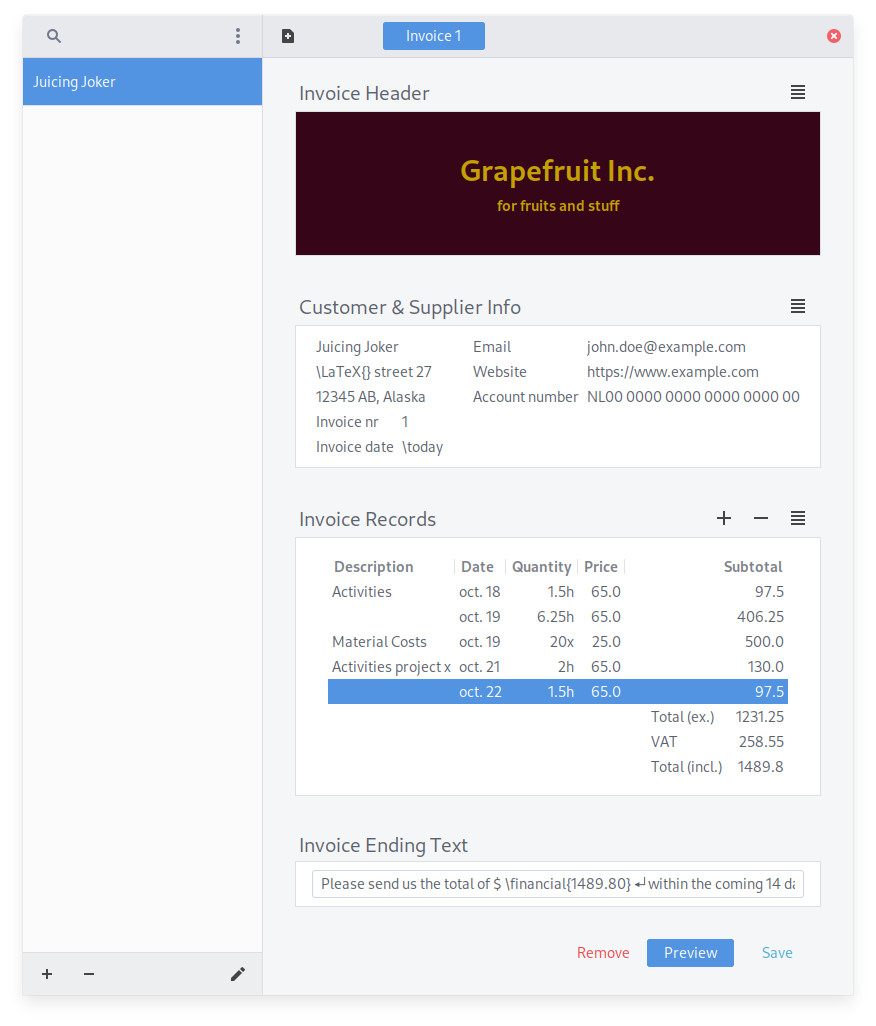
\includegraphics[width=\linewidth]{ginvoice/app.jpg}
    \caption{GinVoice — de applicatie}\label{fig:app}
\end{figure}
Zo zie je de \textit{header}, \textit{informatietabellen}, \textit{factuurregels} en de \textit{slottekst} erin terug komen.
In figuur~\ref{fig:app} kun je zien dat de invoervelden al zijn ingevuld en dat de inhoud daarvan niet veel afwijkt als je het vergelijkt met het eindresultaat, te zien in figuur~\ref{fig:voorbeeldfactuur}.
Er komen later in dit hoofdstuk nog andere applicatie weergaves naar voren.
\begin{figure}[!ht]
    \centering
    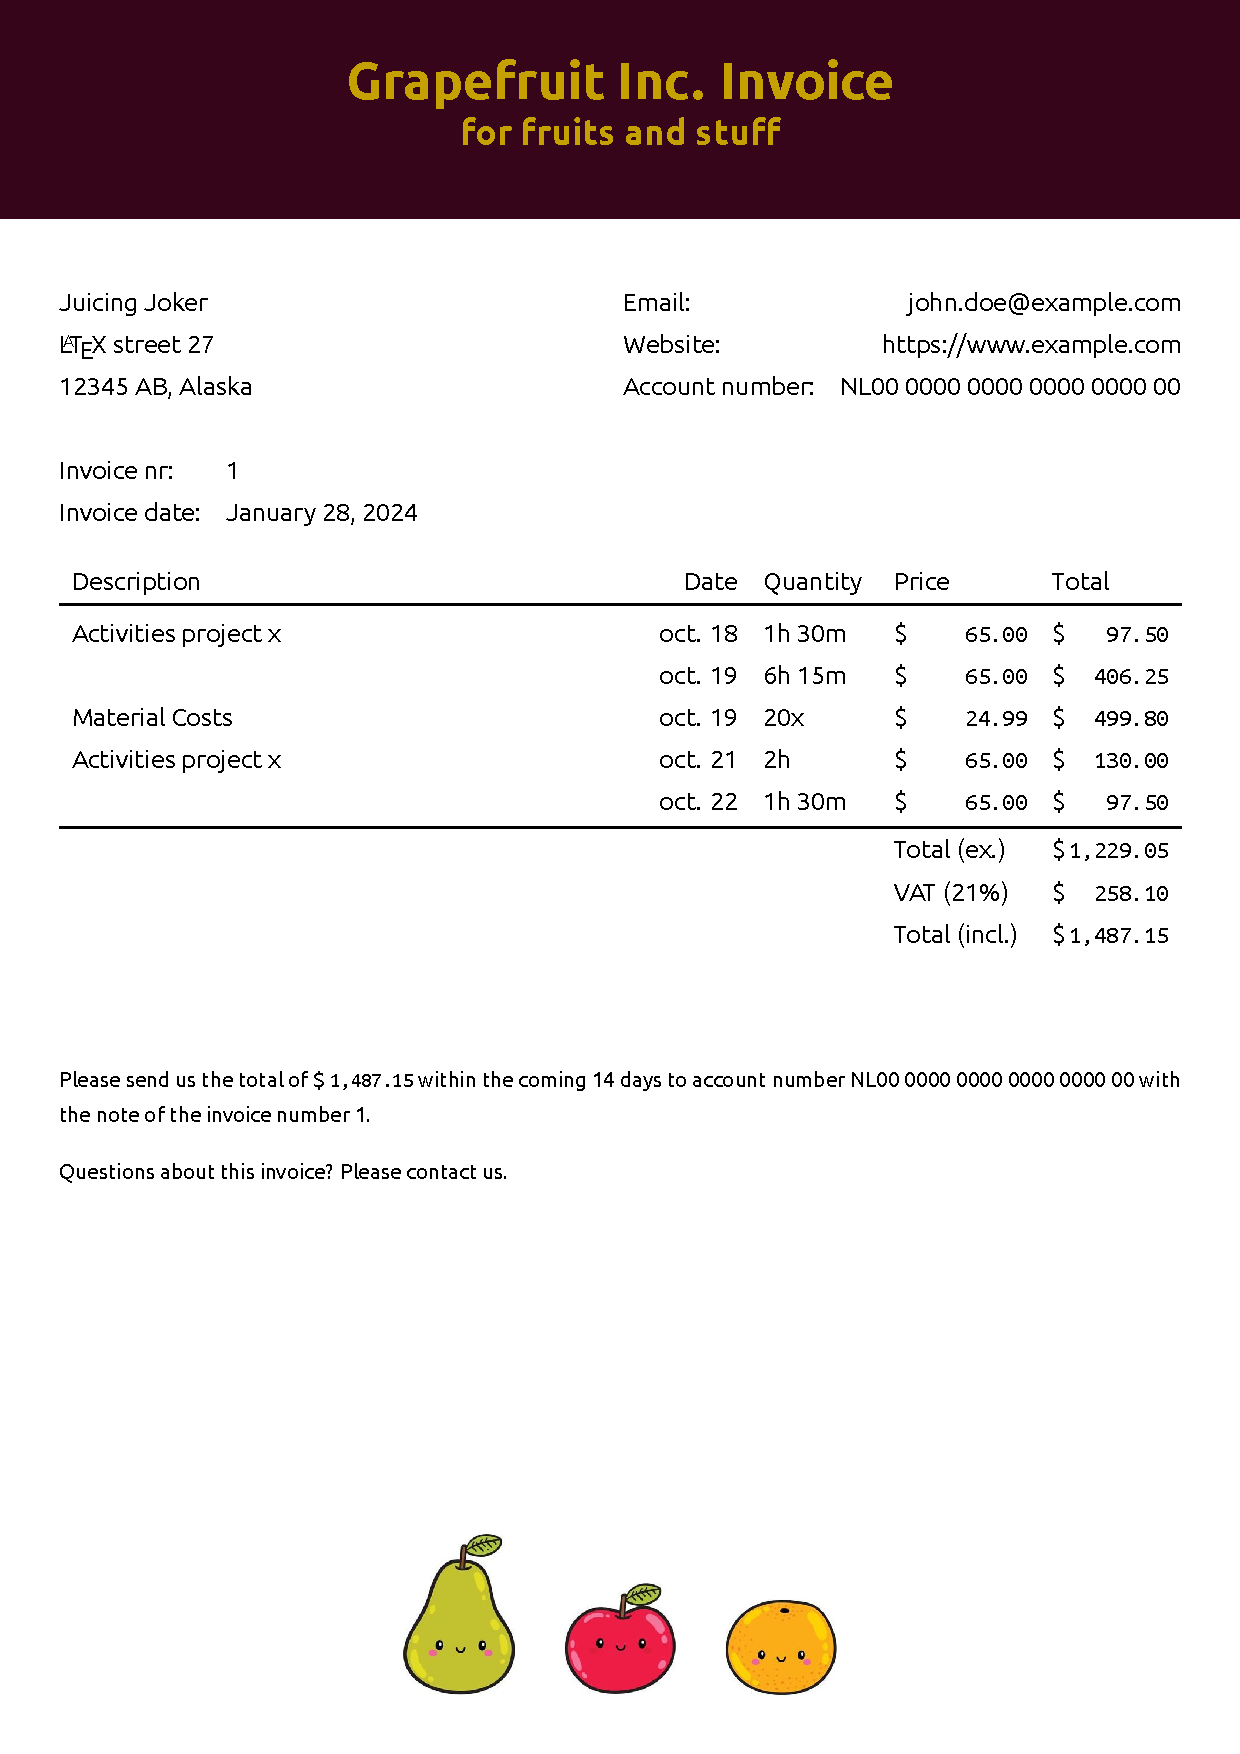
\includegraphics[width=\linewidth]{ginvoice/ginvoice.pdf}
    \caption{Voorbeeldfactuur gegenereerd met GinVoice}
    \label{fig:voorbeeldfactuur}
\end{figure}
\subsection{\LaTeX-template}
Hieronder vind je een voorbeeld van de code binnen de \texttt{document} omgeving:

\lstinputlisting[name=invoice-original,language={[LaTeX]TeX},firstnumber=52,linerange={52-81},numbers=left,xleftmargin=15pt,label={lst:main},caption={\texttt{invoice.tex}}]{ginvoice/invoice-original.tex}

De broncode in listing~\ref{lst:main} demonstreert verschillende macro's die vervangen zullen worden door \pkg{lua-placeholders}, waaronder \cs{title}, \cs{subtitle}, \cs{addressee}, \cs{customerinfo}, \cs{supplierinfo}, \cs{tablefooter}, \cs{tablerecords}, \cs{theending} en \cs{images}.
Daarnaast zijn er variabelen zoals stijl gerelateerde informatie en \cs{currency} die ook behandeld zullen worden.

\subsection{Gegenereerde \LaTeX-bestanden}
Het is belangrijk om te weten dat GinVoice\cite{ginvoice} momenteel een Python script -- \texttt{generator.py} -- gebruikt om extra \TeX-bestanden te genereren.
Deze \TeX-bestanden worden vervolgens in de template ingeladen met \cs{include}, zodat de benodigde macro's beschikbaar zijn.
%Echter, met de introductie van \pkg{lua-placeholders} zal deze aanpak niet langer nodig zijn.

Te beginnen met de taalinstelling:
\begin{figure}[!ht]
    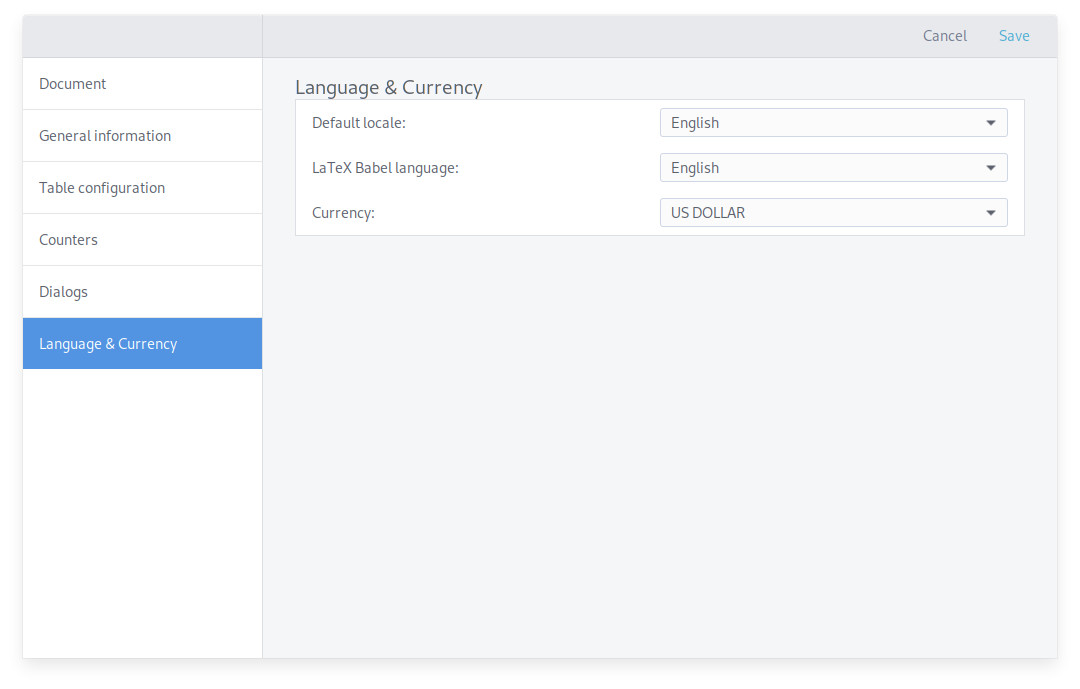
\includegraphics[width=\linewidth]{ginvoice/locale.jpg}
    \caption{Taalinstellingen}\label{fig:locale}
\end{figure}
\lstinputlisting[language={[LaTeX]TeX},caption={\texttt{languages.tex}}]{ginvoice/languages.tex}
Destijds heb ik ervoor gekozen om een aparte taalinstelling in de applicatie op te nemen te zien in figuur~\ref{fig:locale}, zodat woorden binnen de factuur netjes worden afgebroken met behulp van \pkg{babel}.

Een ander aspect binnen de preamble is het instellen van de documenteigenschappen.
Deze macro's komen mee vanuit het gegenereerde bestand \texttt{meta.tex}, waarvan de macro's later in het proces worden gebruikt in de \cs{hypersetup}.
\lstinputlisting[language={[LaTeX]TeX},caption={\texttt{meta.tex}}]{ginvoice/meta.tex}
Veelvoorkomende macro's, zoals \cs{title} worden op meerdere plekken gebruikt.
Dat is dan ook gelijk de reden waarom de \cs{title} niet in de \texttt{header.tex} hoeft te staan.
\lstinputlisting[language={[LaTeX]TeX},caption={\texttt{header.tex}}]{ginvoice/header.tex}
Het adres van de klant wordt in een macro gestopt, waarbij de adresregels van elkaar zijn gescheiden met behulp van een regeleinde.
\lstinputlisting[language={[LaTeX]TeX},caption={\texttt{addressee.tex}}]{ginvoice/addressee.tex}
Deze aanpak zou geschikt zijn voor een tabel met één kolom, of voor bijvoorbeeld een \texttt{enumerate} omgeving.

De informatie van de klant en de leverancier gaat uit van een tabel omgeving met twee kolommen.
\lstinputlisting[language={[LaTeX]TeX},caption={\texttt{customer\_info.tex}}]{ginvoice/customer_info.tex}
\lstinputlisting[language={[LaTeX]TeX},caption={\texttt{supplier\_info.tex}}]{ginvoice/supplier_info.tex}
Het nadeel van deze opzet is dat een en-teken (\&) helemaal geen functie heeft binnen de context van de macro zelf.
Dat zou pas het geval zijn wanneer je binnen een \texttt{tabular} omgeving aan het werk bent.
Los van het feit dat de meeste \LaTeX-editors hierop een foutmelding geven, werkt deze aanpak gek genoeg alsnog.

De meest grote uitdaging binnen de applicatie was het configureerbaar maken van de factuurtabel.
\begin{figure}[!ht]
    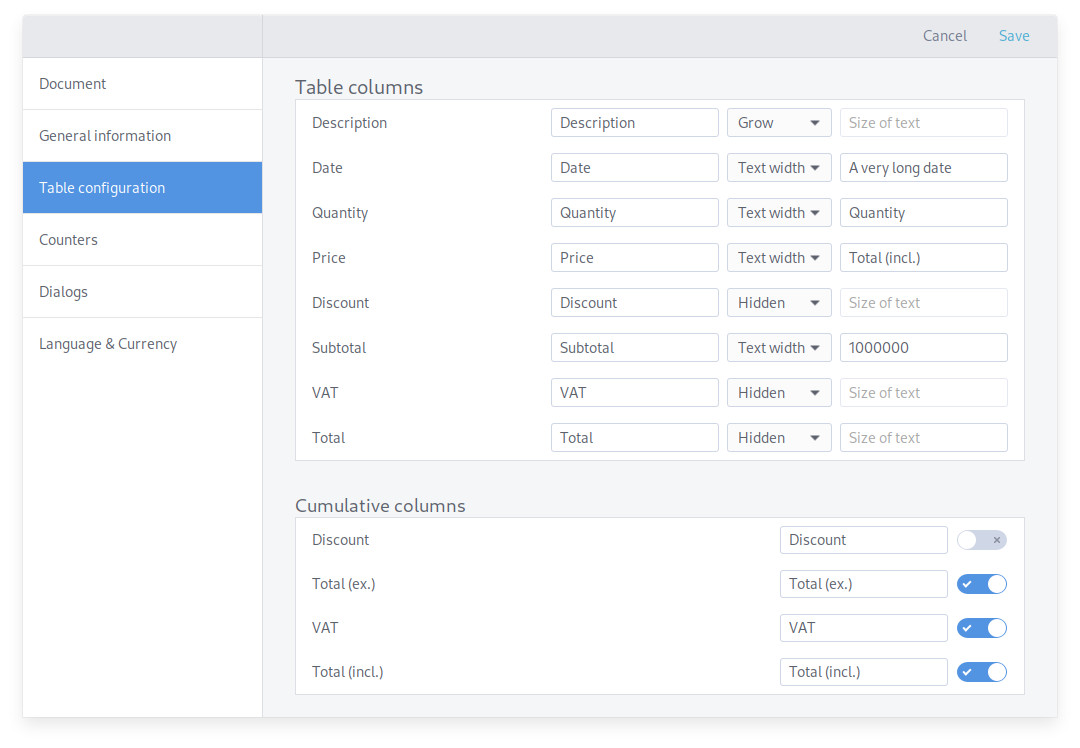
\includegraphics[width=\linewidth]{ginvoice/table-settings.jpg}
    \caption{Tabelinstellingen}\label{fig:tableconfig}
\end{figure}
Hiervoor is een aparte weergave, te zien in figuur~\ref{fig:tableconfig}.
In het figuur zie je dat iedere kolom een andere breedte kan hebben.
Dit kan zijn: de lengte van een stuk tekst, zo groot mogelijk, of verborgen.
Deze toegevoegde complexiteit vanuit de applicatie heeft destijds een behoorlijk complexe uitkomst gehad op het gegenereerde \texttt{table.tex} bestand, te zien in de volgende code:
\lstinputlisting[language={[LaTeX]TeX},caption={\texttt{table.tex}}]{ginvoice/table.tex}
Naast de complexe kolom configuratie heb je \cs{tablerecords} en \cs{tablefooter}, beide vergelijkbaar met bijvoorbeeld de \textit{leveranciersinformatie}.

Het laatste gegenereerde bestand \texttt{footer.tex} definieert de laatst ontbrekende macro's, \cs{theending} en \cs{images}:
\lstinputlisting[language={[LaTeX]TeX},caption={\texttt{footer.tex}}]{ginvoice/footer.tex}
Destijds heb ik er voor gekozen om alle grafische bestanden ergens binnen de omgeving van GinVoice op te slaan.
Dit heb weten te koppelen met \LaTeX\ door gebruik te maken van \cs{graphicspath}.

\subsection{Factuurdata}\label{sec:invoice data}
Als we kijken naar alle informatie afkomstig uit GinVoice, met uitzonderingen daar gelaten, dan komen we uit op de data gepresenteerd in figuur~\ref{fig:klassendiagram}.

\begin{figure}[!ht]
    \centering
    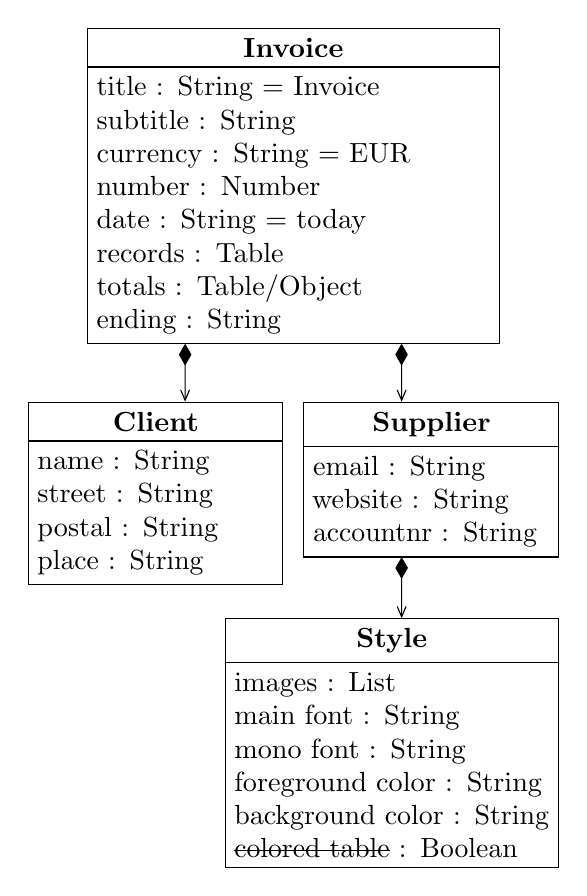
\begin{tikzpicture}
    \begin{class}[text width=5cm]{Invoice}{1.75,0}
        \attribute{title : String = Invoice}
        \attribute{subtitle : String}
        \attribute{currency : String = \cs{EUR}}
        \attribute{number : Number}
        \attribute{date : String = \cs{today}}
        \attribute{records : Table}
        \attribute{totals : Table/Object}
        \attribute{ending : String}
    \end{class}
    \begin{class}[text width=3cm]{Supplier}{3.5,-4.75}
        \attribute{email : String}
        \attribute{website : String}
        \attribute{accountnr : String}
    \end{class}
    \begin{class}[text width=3cm]{Client}{0,-4.75}
        \attribute{name : String}
        \attribute{street : String}
        \attribute{postal : String}
        \attribute{place : String}
    \end{class}
    \begin{class}[text width=4cm]{Style}{3,-7.5}
        \attribute{images : List}
        \attribute{main font : String}
        \attribute{mono font : String}
        \attribute{foreground color : String}
        \attribute{background color : String}
        \attribute{\sout{colored table} : Boolean}
    \end{class}
    \draw[umlcd style, diamond-angle 45] ($(Invoice.south west) - (-1.25,0)$) -- ($(Client.north) + (.375,0)$);
    \draw[umlcd style, diamond-angle 45] ($(Invoice.south east) + (-1.25,0)$) -- ($(Supplier.north) + (-.375,0)$);
    \draw[umlcd style, diamond-angle 45] ($(Supplier.south) + (-.375,0)$) -- ($(Style.north) + (.125,0)$);
\end{tikzpicture}

    \caption{Klassendiagram van de factuur}
    \label{fig:klassendiagram}
\end{figure}

Ik heb voor het gemak alvast alle informatie opgeknipt in aparte entiteiten, die overeen zullen komen met de YAML-bestanden, uitvoerig besproken in hoofdstuk~\ref{sec:new situation}.

%\subsection{Resultaat Voorbeeld}
%Het voorbeeld in figuur~\ref{fig:voorbeeldfactuur} toont een gegenereerde factuur met behulp van de huidige implementatie van GinVoice.
%\begin{figure}[!ht]
%    \centering
%    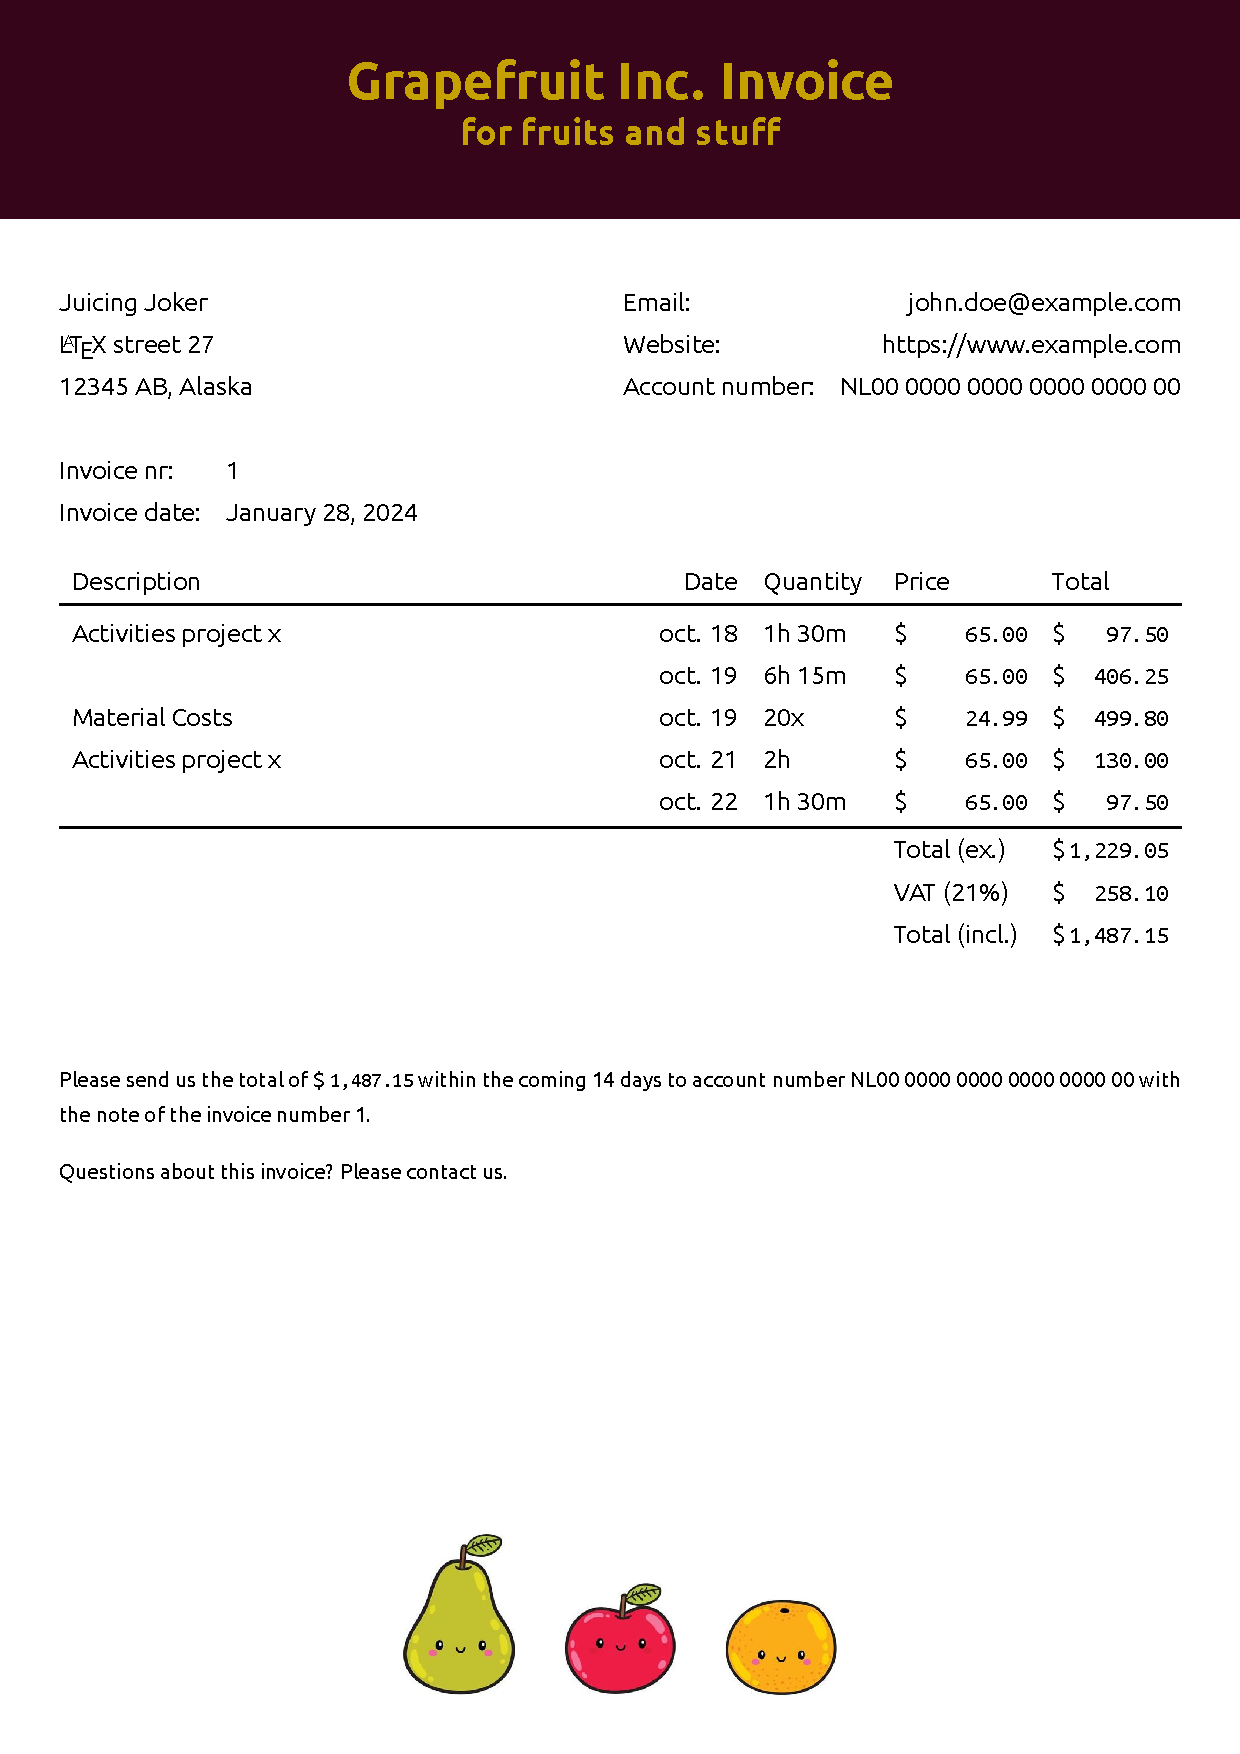
\includegraphics[width=\linewidth]{ginvoice/ginvoice.pdf}
%    \caption{Voorbeeldfactuur gegenereerd met GinVoice}
%    \label{fig:voorbeeldfactuur}
%\end{figure}
%Echter, op dit moment vereist het genereren van dit voorbeeld Python, wat voor template makers die hoofdzakelijk \LaTeX\ gebruiken, ongewenst is.
%In het volgende hoofdstuk zullen we deze situatie aanpakken en laten zien hoe dit voorbeeld rechtstreeks kan worden gegenereerd met \LuaLaTeX.


    \section{YAML Interfaces with \texttt{lua-placeholders}}\label{sec:data}

This chapter demonstrates how YAML interfaces, also known as \textit{recipes}, can be used as interfaces for invoice templates and how they can be integrated into \LaTeX.
The ultimate goal is to provide an efficient and customizable invoicing interface that can be easily integrated into GinVoice.

\subsection{YAML Specifications}
Based on the data analysis in Chapter~\ref{sec:invoice data}, we can start working with the \textit{recipes}.
All \textit{recipes} are placed in the \texttt{recipes} directory relative to the \LaTeX\ project.
Alternatively, you can keep the same directory under \texttt{\$TEXMFHOME/tex/} to make the \textit{recipes} available everywhere.

\subsubsection{The Invoice}
The invoice recipe, \texttt{recipes/invoice.yaml}, specifies two relationships: \texttt{supplier} and \texttt{client}, as indicated in Chapter~\ref{sec:invoice data}.
\lstinputlisting[language=YAML,caption={\texttt{recipes/invoice.yaml}},linerange=1-5,numbers=left,xleftmargin=15pt]{demo/recipes/invoice.yaml}
How the corresponding recipes are loaded based on these values is described in Chapter~\ref{sec:preamble}.

The data within the invoice part can be standardized using a \texttt{default} field, as shown for \texttt{title}.
You can even invoke \LaTeX\ from a default value, including other parameters using \cs{param}.
\lstinputlisting[language=YAML,firstnumber=6,linerange=6-21,numbers=left,xleftmargin=15pt]{demo/recipes/invoice.yaml}
In addition to default values, temporary placeholders can also be specified.

The most complex part of the invoice is the invoice table.
Here, you can specify columns, just as you would for other data types.
\lstinputlisting[language=YAML,firstnumber=22,linerange=22-39,numbers=left,xleftmargin=15pt]{demo/recipes/invoice.yaml}
As mentioned earlier in Chapter~\ref{sec:invoice data}, for most \LaTeX\ users, the \texttt{total} column can be omitted and calculated using packages like \texttt{invoice2}.
Additionally, it would be necessary to make the \texttt{quantity} field of type \texttt{number} and add an extra field like \texttt{quantity type} to specify the correct notation for the \texttt{quantity} column.

For the grand totals, I have chosen the type \texttt{object} so that I can manually place the different totals in \LaTeX.
\lstinputlisting[language=YAML,firstnumber=40,linerange=40-51,numbers=left,xleftmargin=15pt]{demo/recipes/invoice.yaml}
The grand totals could also be handled in a more generic way, such as the \texttt{extra fields} field in the supplier recipe (see Chapter~\ref{sec:supplier spec}).

The last field of the invoice, \texttt{message}, uses a special YAML functionality, namely multiline strings in the default value.
\lstinputlisting[language=YAML,firstnumber=52,linerange=52-,numbers=left,xleftmargin=15pt]{demo/recipes/invoice.yaml}
By using the pipe (\texttt{|}), this mode is activated.
This construction is ideal for large texts, possibly with \LaTeX\ syntax.

\subsubsection{Client}
The client data does not have any special specifications compared to the invoice.
\lstinputlisting[language=YAML,caption={\texttt{recipes/client.yaml}},numbers=left,xleftmargin=15pt]{demo/recipes/client.yaml}
Alternatively, all address details could be specified as a \texttt{list} type, along with a specification, as seen in the \texttt{extra fields} for the supplier.
This would make the interface more generic but less adaptable within the \LaTeX\ context.

\subsubsection{Supplier}\label{sec:supplier spec}
In the case of the supplier recipe, the \texttt{style} field serves the same function as \texttt{supplier} and \texttt{client} in the invoice, allowing the user to choose which style to apply.
\lstinputlisting[language=YAML,caption={\texttt{recipes/supplier.yaml}},numbers=left,xleftmargin=15pt]{demo/recipes/supplier.yaml}

Another interesting field in this specification is \texttt{extra fields}.
This field uses the type \texttt{table} to allow additional information fields, such as the supplier's account number, VAT number, or other relevant details.
Using a table instead of a fixed number of fields gives the end user the flexibility to add as much extra information as needed without imposing limitations.

\subsubsection{Style}
In the style recipe, fonts, colors, and multiple images can be specified.
As mentioned earlier, for \LaTeX\ users, this could be completely omitted and specified directly in \LaTeX\ itself.
\lstinputlisting[language=YAML,caption={\texttt{recipes/style.yaml}},numbers=left,xleftmargin=15pt]{demo/recipes/style.yaml}
Noteworthy is the type for \texttt{images}, namely \texttt{list}.
In Chapter~\ref{sec:typesetting}, it is shown how this list is loaded at the bottom of the invoice.

\subsection{The New Invoice}
Now that the recipes are in order, we can move on to integrating them into \LaTeX.

\subsubsection{Loading Recipes in the Preamble}
The recipes are loaded using the macro \cs{loadrecipe}.
\lstinputlisting[language={[LaTeX]TeX},numbers=left,xleftmargin=15pt,firstnumber=44,linerange=44-47]{demo/invoice.tex}
For the \texttt{invoice} recipe, you can see that it receives the \meta{namespace} \cs{jobname}.
This is because the macro \cs{param} uses \cs{jobname} as the default \meta{name\-space}, simplifying its use.

The other recipes do not specify a \meta{namespace}, meaning they carry the base name of the path as the \meta{namespace}.
In this case, respectively \texttt{supplier}, \texttt{client}, and \texttt{style}.

\subsubsection{Currency}
Regarding the currency, I have chosen to disguise it in the \cs{currency} macro.
This is because it is also used in other files, such as \texttt{invoice.cls}.
\lstinputlisting[language={[LaTeX]TeX},numbers=left,xleftmargin=15pt,firstnumber=49,linerange=49]{demo/invoice.tex}
If the \meta{currency} is not set, the default value from \texttt{style.yaml} is used.
In this case, it defaults to \cs{EUR}.

\subsubsection{Loading Values}\label{sec:preamble}
I manage all YAML files related to the payload in corresponding directories.\\
\dirtree{%
    .1 \meta{project name}.
    .2 recipes.
    .3 \meta{recipe}.yaml.
    .2 invoices.
    .3 \meta{invoice-xxx}.yaml.
    .2 clients.
    .2 \textit{et cetera}.
}
\noindent
Values, also called the payload, are loaded similarly to recipes but with the macro \cs{loadpayload}.
Due to the relationships described in Chapter~\ref{sec:invoice data}, this is slightly more complex than recipes because \pkg{lua-placeholders} does not offer anything standard for this.
\lstinputlisting[language={[LaTeX]TeX},numbers=left,xleftmargin=15pt,firstnumber=51,linerange=51-54]{demo/invoice.tex}
For loading invoice values, it checks if a corresponding YAML file exists.
If so, that payload is loaded, and the experimental macro \cs{strictparams} is used, which will in the future result in errors when mandatory data is missing.

If no corresponding file is found, a default invoice template is compiled.

After loading the invoice data, we check if a client is specified in the invoice data.
We do this using \cs{hasparam}.
It concerns the invoice data, for which we do not need to specify a \meta{namespace}.
\lstinputlisting[language={[LaTeX]TeX},numbers=left,xleftmargin=15pt,firstnumber=56,linerange=56-58]{demo/invoice.tex}
Generally, \cs{param} is not intended for use within the preamble because it can also yield placeholders with \LaTeX\ formatting.
For such tricky situations, the \cs{rawparam} macro is written, as done for the client and supplier.
This macro has no optional arguments, which often causes problems with packages like \texttt{pgfkeys}.

\lstinputlisting[language={[LaTeX]TeX},numbers=left,xleftmargin=15pt,firstnumber=60,linerange=60-62]{demo/invoice.tex}
As seen, loading the supplier does not differ from loading the client.
However, there is still an additional action after loading the supplier, namely checking if the style can be loaded.
This is done in the same way as for the client and supplier themselves, but here you see that the \meta{namespace} must be set.
\lstinputlisting[language={[LaTeX]TeX},numbers=left,xleftmargin=15pt,firstnumber=64,linerange=64-72]{demo/invoice.tex}
For the style-related data, I have chosen to configure the values directly in the corresponding macros, such as \cs{setmainfont} and \cs{definecolor}, as long as a style is specified.
You could also choose to set the style values by default based on the default values specified in the style recipe, by placing the configuration outside the \cs{hasparam} block.

\subsection{Processing in Document}\label{sec:typesetting}
Before we can proceed to compile invoices, we have one task left, namely to set all values in the document itself.
\subsubsection{Header}
As mentioned earlier in Chapter~\ref{sec:legacy-invoice}, the \cs{makeheader} macro comes from \texttt{invoice.cls}.
For now, let's assume that \texttt{invoice.cls} has been modified so that it no longer causes errors and that \cs{makeheader} now expects the title and subtitle as arguments:
\lstinputlisting[language={[LaTeX]TeX},numbers=left,xleftmargin=15pt,firstnumber=76,linerange=76-79]{demo/invoice.tex}
In the example, there are only two differences compared to the old version, namely:\\
\cs{title}\hfill\textrightarrow\hfill\lstinline[language={[LaTeX]TeX}]|\param{title}|\\
\cs{subtitle}\hfill\textrightarrow\hfill\lstinline[language={[LaTeX]TeX}]|\param{subtitle}|\\
However, this time correctly passed to the \texttt{document\-class}.

\subsubsection{Information}
The left column of the information is quite tricky, as it contains both client information and invoice data such as number and date.
\lstinputlisting[language={[LaTeX]TeX},numbers=left,xleftmargin=15pt,firstnumber=80,linerange=80-91]{demo/invoice.tex}
You can see in the address lines that each line is terminated with a line break.
This could have also been achieved if, for example, there was a \texttt{address lines} field of type \texttt{list}.
Then, with \lstinline|\param[client]{address lines}|, that would have been solved in one go, given that \texttt{postal} and \texttt{place} are combined on one line in YAML\@.
The mentioned alternative assumes that the \cs{paramlistconjunction} macro is set to `\texttt{\textbackslash\textbackslash}', instead of the default value `\texttt{,\~}'.
\lstinputlisting[language={[LaTeX]TeX},numbers=left,xleftmargin=20pt,firstnumber=92,linerange=92-101]{demo/invoice.tex}
The right column of information is similar to the left, but it has an additional special field, namely \texttt{extra fields} of type \texttt{table}.
This allows adding a variable number of rows.
The same could potentially be applied to the client data in the left column.
Then it only remains to choose whether to place them above or below the invoice information.

\subsubsection{Table}
As mentioned earlier, standardizing the column definition is difficult.
On line 105, you can see what the \cs{columdefs} could have provided, except for the counters I used earlier.
\lstinputlisting[language={[LaTeX]TeX},numbers=left,xleftmargin=20pt,firstnumber=103,linerange=103-105]{demo/invoice.tex}
For the second argument of the \texttt{invoice} environment, a static header is set.
\lstinputlisting[language={[LaTeX]TeX},numbers=left,xleftmargin=20pt,firstnumber=106,linerange=106-107]{demo/invoice.tex}
For the third argument of the \texttt{invoice} environment, you can see how the grand totals are set in the table.
These totals are placed in the last two columns of each row, so that they align neatly with the rest of the table.
\lstinputlisting[language={[LaTeX]TeX},numbers=left,xleftmargin=20pt,firstnumber=108,linerange=108-113]{demo/invoice.tex}
In the final part of the table, you can see how each invoice item is set using \cs{formatrecords} and \cs{fortablerow}.
\lstinputlisting[language={[LaTeX]TeX},numbers=left,xleftmargin=20pt,firstnumber=114,linerange=114-119]{demo/invoice.tex}
The overall structure of the table still comes from the previous situation.
The notable difference compared to the new situation is that the data can be placed in all sorts of table structures since the data is decoupled from the \LaTeX\ and application domain, and the typesetting challenges are shifted to the \LaTeX\ domain.

\subsubsection{Closing Text and Images}
Where we previously saw an advanced YAML specification for the \texttt{message} field, the implementation within \LaTeX\ remains almost the same:
\lstinputlisting[language={[LaTeX]TeX},numbers=left,xleftmargin=20pt,firstnumber=121,linerange=121]{demo/invoice.tex}
The only difference is:\\
\cs{theending}\hfill\textrightarrow\hfill\lstinline|\param{message}|\\
However, for the images, it's a bit trickier to implement in \LaTeX\ due to the \texttt{list} type.
\lstinputlisting[language={[LaTeX]TeX},numbers=left,xleftmargin=20pt,firstnumber=122,linerange=122-]{demo/invoice.tex}
Where previously in Python, all images were neatly placed side by side, with a \cs{hspace} of \texttt{1.5em} between each image, I chose to apply half of that as \cs{hspace} on both sides of each image.
This is because the \cs{forlistitem} macro does not yet have a convenient way to do this, like \cs{param} does by setting \cs{paramlistconjunction} to `\lstinline|\hspace{1.5em}|'.


    \section{Execution}\label{sec:output}
% Advanced YAML payload examples, + sequence diagram command line
Now that the legacy invoice has been completely transformed, let's see what the result looks like.
If you want to participate via the command line, please refer to the full source code\cite{ginvoice-template} of these examples.

\subsection{The Template Version}
Without providing any values, we get the following result, as shown in figure~\ref{fig:template}.\\
\setlength\fboxsep{0pt}%
\begin{figure}[!ht]%
    \fbox{\includegraphics[width=\linewidth-1pt]{invoice-template.pdf}}%
    \caption{\texttt{invoice-template.pdf}}\label{fig:template}%
\end{figure}
As mentioned earlier, \pkg{lua-placeholders} can only be compiled with \LuaLaTeX.
Additionally, the option \texttt{--shell-escape} is required to load YAML files.
The example can be compiled as follows:
\begin{lstlisting}[language=bash,caption={Compiling with \texttt{lualatex}}]
lualatex --shell-escape \
     --jobname=invoice-template \
     --output-directory=$(OUTPUT_DIR) \
       invoice
\end{lstlisting}
Where \texttt{\$(OUTPUT\_DIR)} is the desired output directory.

However, if you are designing a template, continuous generation with \LaTeX\ MK is more user-friendly:
\begin{lstlisting}[language=bash,caption={Compiling with \texttt{latexmk}}]
latexmk -pvc -lualatex \
    --shell-escape \
    --jobname=invoice-template \
    --output-directory=$(OUTPUT_DIR) \
      invoice
\end{lstlisting}
This way, you don't have to recompile with \TeX\ every time there is a change; it happens automatically.

\subsection{YAML Values}
To get a filled invoice, we will need the following YAML files:

\dirtree{%
    .1 \meta{project dir}.
    .2 invoices.
    .3 \meta{invoice}.yaml.
    .2 suppliers.
    .3 \meta{supplier}.yaml.
    .2 styles.
    .3 \meta{style}.yaml.
    .2 clients.
    .3 \meta{client}.yaml.
}

This structure is based on the implementation described in section~\ref{sec:preamble}.
Before discussing the contents of the YAML files, we can first consider alternative project structures.

\subsubsection{Alternative Project Structure}
Everyone is free to create their desired folder structure.
For example, you could place styles under\\
\hspace*{4em}\texttt{/suppliers/\meta{supplier}/style.yaml}\\
so that you can even omit the \texttt{style} field in the supplier recipe.
Another option is to place the \texttt{clients} folder under the supplier level, so you don't accidentally mix clients of different suppliers.
This could be achieved as follows:
\dirtree{%
    .1 \meta{project dir}.
    .2 suppliers.
    .3 \meta{supplier}.yaml.
    .3 \meta{supplier}.
    .4 \meta{client}.yaml.
}
\noindent
This way, the implementation for loading clients would require the variables \meta{supplier} and \meta{client}, to then reach the path\\
\hspace*{4em}\texttt{suppliers/\meta{supplier}/\meta{client}.yaml}.

The same consideration could be applied to the invoices, but this is a more difficult scenario, as the invoice data is based on the \cs{jobname} in the implementation of section~\ref{sec:preamble}.
One possible solution for this is to manage the project per supplier.
You can then place the \textit{recipes} in the \texttt{\$TEXMFHOME/tex} directory so that they are available for all projects.
Here's an example of a possible project structure:\\
\begin{minipage}{.49\linewidth}
\dirtree{%
    .1 \$HOME/texmf/tex.
    .2 recipes.
    .3 invoice.yaml.
    .3 client.yaml.
    .3 supplier.yaml.
    .3 style.yaml.
    .2 invoice.cls.
    .2 invoice.tex.
}
\end{minipage}%
\hfill
\begin{minipage}{.49\linewidth}
\dirtree{%
    .1 \meta{project dir}.
    .2 invoices.
    .3 \meta{invoice}.yaml.
    .2 clients.
    .3 \meta{client}.yaml.
    .2 supplier.yaml.
    .2 style.yaml.
}
\end{minipage}
In this example, all data is separated per supplier, including client information and final invoices.

\subsection{Suppliers and Clients}\label{sec:supplier and client}
In the example result of GinVoice, a client \textit{Juicing Joker} was shown.
In YAML, this would translate to:
\lstinputlisting[captionpos=b,caption={\texttt{clients/juicing-joker.yaml}}]{demo/clients/juicing-joker.yaml}

This way, the client can be referenced in the invoice with \texttt{juicing-joker}.

For the supplier, we saw \textit{Grapefruit Inc.} in the example, which translates to:
\lstinputlisting[captionpos=b,caption={\texttt{suppliers/grapefruit.yaml} or \texttt{grapefruit/supplier.yaml}}]{demo/suppliers/grapefruit.yaml}

And for the style:
\lstinputlisting[captionpos=b,caption={\texttt{styles/grapefruit.yaml} or \texttt{grapefruit/style.yaml}}]{demo/styles/grapefruit.yaml}

The advantage of the alternative project structure is that \texttt{invoice-template} automatically picks up the styling as well as the supplier information, as seen in figure~\ref{fig:result alt}.

\onecolumn
\subsection{Invoices}
\begin{figure}[!ht]
%    \centering
    \begin{subfigure}{.32\linewidth}
        \fbox{\includegraphics[width=\linewidth-1pt]{invoice2-template.pdf}}
        \caption{\texttt{invoice-template.pdf}}\label{fig:result alt}
    \end{subfigure}\hfill
    \begin{subfigure}{.32\linewidth}
        \fbox{\includegraphics[width=\linewidth-1pt]{invoice-001.pdf}}
        \caption{\texttt{invoice-001.pdf}}\label{fig:result 1}
    \end{subfigure}\hfill
    \begin{subfigure}{.32\linewidth}
        \fbox{\includegraphics[width=\linewidth-1pt]{invoice-002.pdf}}
        \caption{\texttt{invoice-002.pdf}}\label{fig:result 2}
    \end{subfigure}
    \caption{Invoice Examples}\label{fig:pdfs}
\end{figure}
\begin{multicols}{2}
    \noindent
    To create an invoice that exactly matches the standard example of GinVoice, as seen in figure~\ref{fig:result 1}, we use the following YAML example:
    \lstinputlisting[xleftmargin=15pt,numbers=left,linerange=-15,caption={\texttt{invoices/invoice-001.yaml}}]{demo/invoices/invoice-001.yaml}
    The actors \texttt{grapefruit} and \texttt{juicing-joker}, discussed in section~\ref{sec:supplier and client}, are seen in the invoice.
Additionally, the example has the same general information to achieve the same result.
In the \texttt{records} field, you can see that one row of the table takes up many lines.
In the second row of the table, you can see that the \texttt{description} field has an empty value.
    \columnbreak
    If the quotes are omitted in YAML, you will get an error when converting to data.
Since the rows do not differ too much from each other, we continue the example at the \texttt{totals} field:
    \lstinputlisting[xleftmargin=15pt,numbers=left,linerange=34-,firstnumber=34]{demo/invoices/invoice-001.yaml}
    Lastly in the example, we see the totals and the closing text.

    This invoice can then be compiled with the following command:
    \begin{lstlisting}[language=bash]
lualatex --shell-escape \
    --jobname=invoice-001 \
    --output-directory=$(OUTPUT_DIR) \
      invoice
    \end{lstlisting}
%    The only difference between compiling the template version is the \cs{jobname}.
\end{multicols}
\twocolumn


    \section{Conclusion}\label{sec:conclusion}

In this article, we have explored how YAML interfaces can be used as a flexible and customizable way to manage and integrate invoice templates in \LaTeX.
By utilizing YAML files for specifying \textit{recipes} and invoice data, we have presented a structured approach for generating invoices using \LuaLaTeX\ and the \pkg{lua-placeholders} package.

Our approach enables easy customization and management of invoice templates, providing users with complete control over the layout and content of the invoices.
Furthermore, we have considered alternative project structures that can further enhance the flexibility and management of invoice templates.

The \pkg{lua-placeholders} package has played a crucial role in optimizing the document interface by providing a powerful and flexible mechanism for replacing variables in \LaTeX\ documents.
By leveraging \LuaLaTeX, users can benefit from the speed and efficiency of Lua for data processing while still enjoying the typographic precision of \LaTeX\ for generating professionally looking documents.

For applications like GinVoice, this approach offers significant benefits as users can now more easily create and execute \LaTeX\ invoice templates and potentially integrate them with the application interface.

We encourage our readers to explore and implement \pkg{lua-placeholders} in their own projects.
The possibilities for system integration and document interfacing with \pkg{lua-placeholders} are extensive, providing users with the flexibility to manage complex document workflows with minimal effort.
By using \pkg{lua-placeholders}, users can enhance the efficiency of their document processes while maintaining the quality and consistency of their documents.

It is also important to consider some considerations for others considering using this package.
While \pkg{lua-placeholders} is a powerful tool for document interfacing, it requires a certain level of familiarity with YAML and \LaTeX.
In the case of the alternative project structure, basic knowledge of the TDS (\TeX\ Directory Structure) is also required.

Finally, we have compared with alternative methods and determined that \pkg{lua-placeholders} is the best choice due to its flexibility, speed, and integration capabilities with \LaTeX.
While there are other approaches to generating documents using \LaTeX, \pkg{lua-placeholders} offers a unique combination of functionality and ease of use, making it an attractive option for document interfacing.

Overall, our research provides a practical and efficient solution for managing and integrating invoice templates in \LaTeX\ projects, allowing users to benefit from a seamless workflow for invoicing and reporting.


    \bibliographystyle{tugboat}%
    \bibliography{references}

    \makesignature
\end{document}
